\section{Implementación}
Hemos realizado una implementación de los algoritmos anteriormente descritos.
Esta implementación tiene la función meramente didáctica de comprobar los
resultados de los distintos algoritmos bajo la elección de distintas matrices
base.

Para la implementación nos hemos decantado por \textbf{Python} como lenguaje de
programación, junto con el framework \textbf{Kivi} que facilita la
implementación de interfaces gráficas y permite correr la aplicación en varias
plataformas fácilmente sin modificaciones en el código (en concreto Linux,
Windows, iOS y Android).

\newpage
\subsection{Características}
\begin{figure}[h]
	\centering
	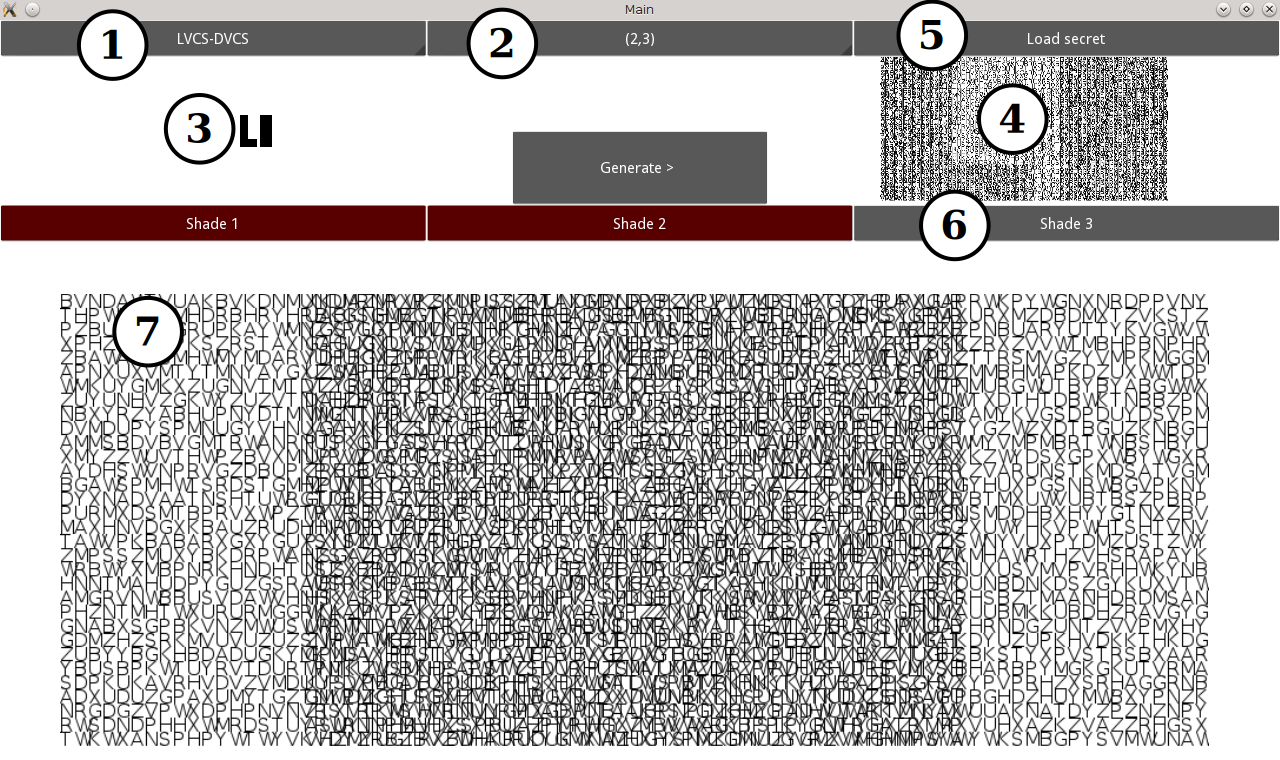
\includegraphics[width=0.9\textwidth]{images/programa}
	\caption{Captura del programa. Se enumeran las características que se
	describen a continuación.}
	\label{fig:programa}
\end{figure}

\begin{enumerate}
	\item \textbf{Selección de algoritmo a utilizar} (DVCS, LVCS-DVCS,
		LVCS-PVCS).
	\item \textbf{Selección de las matrices base a utilizar} ((2,2), (2,3),
		(3,3))
	\item \textbf{Miniatura de la imagen original}
	\item \textbf{Miniatura de la imagen resultado}
	\item \textbf{Carga de la imágen original}
	\item \textbf{Elección de sombras mostradas:} Permite seleccionar las
		sombras que se mostraran en la zona de composición de sombras.
	\item \textbf{Zona de composición de sombras:} Permite arrastra las
		sombras horizontalmente para superponerlas de forma manual.
\end{enumerate}

\subsection{Detalles}
A continuación vamos a explicar ciertos detalles de la implementación, así como
algunos inconvenientes encontrados durante su realización.

\subsubsection{Generación de matrices base}
\label{sec:impl.matrices_base}
Como ya hemos comentado, la generación de matices base que cumplan
correctamente las restricciones es un problema complejo (ver
\cite{generacion_matrices}).

Otro problema añadido a la búsqueda de esta matrices es que la mayoría, aunque
cumplan las restricciones, muestran una diferencia entre los superpíxeles
blancos y negros (contraste) muy leve. Esto hace que las imágenes resultantes
del algoritmo LVCS sean difícilmente apreciables si se utilizan estas matrices.
A partir de $K=3$ nos ha sido imposible encontrar matrices que presenten una
diferencia entre superpíxeles blancos y negros de más de un píxel (ie. $h-l =
1$ ver \refcont{sec:matrices_base}).

Nosotros hemos optado por algoritmos de búsqueda en profundidad con poda para
buscar matrices alternativas a las que se nos proporcionaban en los artículos.
Estos algoritmos nos han proporcionado algunas matrices pequeñas que cumplen las
restricciones, pero resultan inviables a la hora de buscar matrices mayores o
que otorguen un mayor contraste.

\subsubsection{Antialiasing y zoom}
El framework que hemos utilizado realiza antialiasing a las imágenes
automáticamente. Esto ha creado divertidos efectos al superponer las sombras,
pero también impide que se aprecien los resultados si el zoom no es el adecuado.
Hay que tener en cuenta que el zoom digital conlleva una pérdida de información,
si se realiza antes de superponer las sombras, la superposición no será
efectiva.

\subsubsection{Resolución de resultados}
La resolución de las imágenes resultantes por el algoritmo LVCS crece mucho en
relación a la imagen original. Esto es debido a que cada píxel de la imagen
original se sustituye por varias letras que van a ocupar varios píxeles cada una
en la imagen resultado. Esto provoca realentizaciones y agotamiento de memoria
para imágenes grandes en nuestra implementación.
